\subsection{Blazemark}
Blazemark is a benchmark suite provided by Blaze to compare the performance of Blaze with other linear algebra libraries including Blitz++\cite{Blitz}, Boost uBLAS\cite{Boost}, GMM++\cite{GMM++}, Armadillo\cite{sanderson2016armadillo}, MTL4\cite{MTL}, and Eigen3\cite{Eigen}, alongside plain BLAS libraries like Atlas\cite{ATLAS}, Goto\cite{gotoblas}, and Intel MKL.\cite{MKL}

\begin{figure}[H]
	\centering
	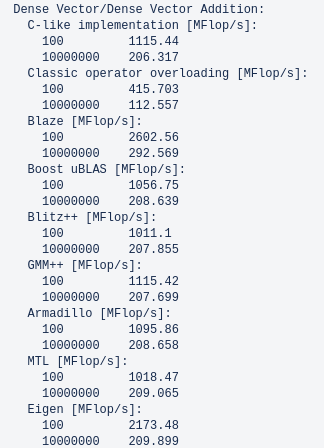
\includegraphics[scale=0.5]{images/blazemark_1.png}
	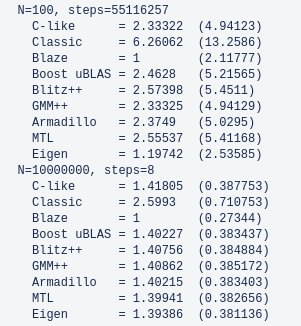
\includegraphics[scale=0.5]{images/blazemark_2.png}
	\caption{An example of the results obtained from running $DVECDVECADD$ benchmark through Blazemark}	
	\label{blazemark1}
\end{figure}


\subsection{Configurations}
Our experiments were run on Marvin nodes of Rostam cluster at Center for Computation and Technology(CCT) at Louisiana State University. Table~\ref{table3} and Table~\ref{table4} show some of the specifications of this node.

\vspace{\baselineskip}	
\begin{table}[H]
	\centering
%	\resizebox{\textwidth}{!}
	\scalebox{0.75}
	{\begin{tabular}{|c | c |} 
			\hline

			Category & Specification\\
			\hline
			\hline
			CPU &  2 x Intel(R) Xeon(R) CPU E5-2450 0 @ 2.10GHz \\ [0.5ex] 
			\hline
			RAM & 48 GB\\ 	
			\hline
			Number of Cores & 16\\
			\hline	
			Hyperthreading & Off \\
			\hline			
	\end{tabular}}	
	\caption{Specifications of the Marvin node from Rostam cluster at CCT.}
	\label{table3}
\end{table} 


\vspace{\baselineskip}	
\begin{table}[H]
	\centering
	\scalebox{0.9}
	{\begin{tabular}{|c | c | c | c | c|} 
			\hline
			Cache Level &  Coherency Line Size & Number of Sets & Ways of Associativity & Size\\ [0.5ex] 
			\hline
			\hline
			1 & 64 & 512 & 8 & 32KB \\	
			\hline
			2 & 64 & 512 & 8 & 256KB \\
			\hline	
			3 & 64 & 512 & 20 & 20480KB \\
			\hline			
	\end{tabular}}	
	\caption{Cache specifications of the Marvin node from Rostam cluster at CCT.}
	\label{table4}
\end{table} 
\vspace{\baselineskip}	

\vspace{\baselineskip}	
\begin{table}[H]
	\centering
	%	\resizebox{\textwidth}{!}
	\scalebox{0.75}
	{\begin{tabular}{|c | c |} 
			\hline
			Library & Version \\
			\hline
			\hline
			HPX & 1.3.0 \\ 
			\hline
			Blaze & 3.5\\ 	
			\hline
			
	\end{tabular}}	
	\caption{Specifications of the libraries used to run our experiments.}
	\label{table5}
\end{table}
%Marvin:
%cache level 1
%coherency line size: 64
%number of sets: 512
%ways of associativity: 8
%type: Instruction
%size: 32K
%
%cache level 2
%coherency line size: 64
%number of sets: 512
%ways of associativity: 8
%type: Unified
%size: 256K
%
%cache level 3
%coherency line size: 64
%number of sets: 512
%ways of associativity: 20
%type: Unified
%size: 20480K
%
%
%Trillian:
%cache level 1
%coherency line size: 64
%number of sets: 64
%ways of associativity: 4
%type: Data
%size: 16K
%
%cache level 1
%coherency line size: 64
%number of sets: 512
%ways of associativity: 2
%type: Instruction
%size: 64K
%
%cache level 2
%coherency line size: 64
%number of sets: 2048
%ways of associativity: 16
%type: Unified
%size: 2048K

%cache level 3
%coherency line size: 64
%number of sets: 2048
%ways of associativity: 48
%type: Unified
%size: 6144K


